\documentclass[Orbiter Developer Manual.tex]{subfiles}
\begin{document}

\section{Basics of orbital mechanics}
This section of the manual contains a very brief summary of basic celestial mechanics.\\
It is intended to clarify some of the concepts of various API functions in this reference document, but may also provide some useful general information for beginners.


\subsection{Elliptic orbits}% TODO fix repeated names
This subsection provides a summary of parameters for ideal 2-body orbital elements.\\
\textbf{Conic section:} The trajectory of an object under the influence of the gravitational field generated by a point mass follows a conic section. This may be either periodic (closed circular or elliptic orbit) or nonperiodic (open parabolic or hyperbolic orbit). The equation of a conic section with the focus in the origin is given in polar coordinates by

\[ r = \frac{p}{1+e \cos(\nu)} \]

\noindent
with eccentricity e and \textit{semi-latus rectum} p.\\
\textbf{Standard gravitational parameter:} In the following, the standard gravitational parameter is defined as the product of the gravitational constant G and the mass M of the central body at focus F:
\[ \mu = GM \]


\subsubsection{Elliptic orbits}% TODO fix repeated names
Elliptic (closed) orbits are characterised by an eccentricity e < 1. A special case are circular orbits (e = 0).

\begin{figure}[H]
  \centering
  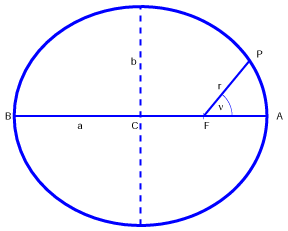
\includegraphics[width=0.5\hsize]{ellips.png}
  \caption{Elliptical orbit with central body at focus F}
\end{figure}

\noindent
\textbf{Semi-major axis (a):} The longest semi-diameter of the ellipse. The distance from the centre (C) through one of the foci (F) to the edge of the ellipse (A). The semi-major axis can be calculated from the parameters of the conic section as
\[ a = \frac{p}{1-e^2} \]

\noindent
\textbf{Semi-minor axis (b):} The shortest semi-diameter of the ellipse. The distance from the centre (C) to the edge of the ellipse, at right angles to the major axis. The semi-minor axis can be calculated from the parameters of the conic section as
\[ b = \frac{p}{\sqrt{1-e^2}} = a \sqrt{1-e^2} \]

\noindent
\textbf{Periapsis:} The periapsis (A) (perigee for Earth orbits, perilune for lunar orbits) is the lowest point of the orbit, i.e. the point of the ellipse closest to focus F. The periapsis distance $r_{pe}$ = FA is given by
\[ r_{\mathrm{pe}} = \frac{p}{1+e} = (1-e)a \]

\noindent
\textbf{Apoapsis:} The apoapsis (B) (apogee for Earth orbits, apolune for lunar orbits) is the highest point of the orbit, i.e. the point of the ellipse farthest from focus F. The apoapsis distance $r_{ap}$ = FB is given by
\[ r_{\mathrm{ap}} = \frac{p}{1-e} = (1+e)a \]

\noindent
\textbf{True anomaly:} The true anomaly (v) of an orbiting object (P) is the angle AFP between P and periapsis A, measured at F.

\noindent
\textbf{Orbital period:} According to Kepler's third law, the square of the period T of an orbiting body is proportional to the cube of the semi-major axis a of the orbit. T is given by
\[ T = 2\pi \sqrt{\frac{a^3}{\mu}} \]

\noindent
\textbf{Orbital speed:} The orbital speed v as a function of radius r is given by
\[ v = \sqrt{\mu\left(\frac{2}{r} - \frac{1}{a}\right)} \]

\noindent
Maximum and minimum speed occur at periapsis and apoapsis, respectively:
\[ v_\mathrm{pe} = \sqrt{\frac{(1+e)\mu}{(1-e)a}}, \qquad v_\mathrm{ap} = \sqrt{\frac{(1-e)\mu}{(1+e)a}} \]

\noindent
The mean orbital speed is given by
\[ \bar{v} = \frac{2\pi a}{T} = \sqrt{\frac{\mu}{a}} = na \]

\noindent
where the mean angular motion \textit{n} is defined as
\[ n = \frac{2 \pi} {T} \]

\noindent
\textbf{Specific orbital energy:} (or vis-viva energy) E is the sum of potential energy $E_{p}$ and kinetic energy $E_{k}$ of an orbiting body. E is constant along the orbit:
\[ E = E_k + E_p = \frac{v^2}{2} - \frac{\mu}{r} = -\frac{1}{2} \frac{\mu^2}{h^2} (1-e^2) \]

\noindent
where h is the specific angular momentum of the orbiting body.

For specific types of orbit, E is given by
\[
E = \left\lbrace \begin{array}{cll}
-\frac{\mu}{2a} & \mathrm{if} & e < 1 \\
0 & \mathrm{if} & e = 1 \\
\frac{\mu}{2a} & \mathrm{if} & e > 1
\end{array}\right.
\]


\subsection{The orbit in space}

The orientation of the orbital trajectory in space, relative to the reference body, is defined by three parameters (in addition to the two parameters describing the shape):
\begin{itemize}
\item inclination
\item longitude of ascending node
\item longitude of periapsis
\end{itemize}

\noindent
The position of the orbiting object along the orbit is defined by an additional parameter, the true longitude.

\begin{figure}[H]
  \centering
  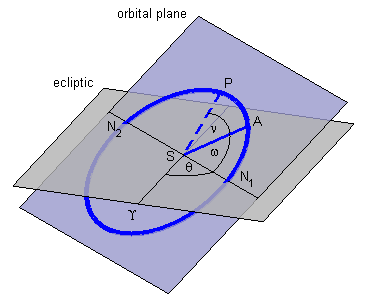
\includegraphics[width=0.5\hsize]{orbit.png}
  \caption{The orbit in space}
\end{figure}

\noindent
The orientation of an orbit in space is defined with respect to a frame of reference. For planetary orbits, the reference is usually given by the plane of the ecliptic and direction of the vernal equinox. For satellites in Earth orbit, the equatorial plane usually defines the reference plane.\\
\textbf{Inclination}: The inclination i defines the tilt of the orbital plane against the reference plane. The intersection of the orbital plane with the reference plane is denoted as the \textit{line of nodes}.\\
\textbf{Ascending and descending node}: The line of nodes always passes through the orbit reference body (S).
The nodes $N_{1}$ and $N_{2}$ are the points where the orbital trajectory intersects the reference plane. If the direction of orbit is such that the orbiting body passes the plane of the ecliptic from south to north at $N_{1}$, then $N_{1}$ is the \textit{ascending node}, and $N_{2}$ is the \textit{descending node}.\\
\textbf{Longitude of ascending node}: The angle between the reference direction $\Upsilon$ and node $N_{1}$ is the \textit{longitude of the ascending node} ($\theta$).\\
\textbf{Argument of periapsis}: The angle between node $N_{1}$ and periapsis A is the \textit{argument of periapsis} ($\omega$).\\
\textbf{Longitude of periapsis}: The sum $\varpi = \theta + \omega$ is called the \textit{longitude of periapsis}.\\
\textbf{True longitude}: The sum of longitude of periapsis and true anomaly,
\[ L = \varpi + \nu = \theta + \omega + \nu \]

\noindent
is called the \textit{true longitude} of the orbiting body.


\subsubsection{Mean longitude}
Consider a vector originating in S and moving in the plane of the orbit with mean angular velocity n, passing through point A at time $t_{0}$.\\
\textbf{Mean anomaly}: At time t, the vector is located at \textit{mean anomaly} $ M = n(t-t_0) $ relative to periapsis A.\\
\textbf{Mean longitude}: The \textit{mean longitude} of the orbiting body is the sum of mean anomaly and longitude of periapsis:
\[ l = \theta + \omega + n(t-t_0) = \varpi + n(t-t_0) \]

\noindent
The \textit{mean longitude at the epoch} is defined as the mean longitude at t=0, given by
\[ \varepsilon = \varpi - nt_0 \]

\noindent
The mean longitude can then be written as
\[ l = nt + \varepsilon \]

\noindent
The mean anomaly is given by
\[ M = n(t-t_0) = l - \varpi = nt + \varepsilon - \varpi \]


\subsection{Kepler's equation}
\subsubsection{True and eccentric anomaly}
To find the position P of an orbiting body at some time t, we need to find its true anomaly $\nu$ at that time. Calculating true anomaly is not trivial for eccentric orbits, because the velocity of the orbiting body is continually changing.\\
\textbf{Eccentric anomaly}: Define a circle with radius \textit{a} (semi-major axis of the orbit ellipse) whose centre coincides with the centre of the ellipse.
Project object position P perpendicular to the semi-major axis onto the circle (Q). Then the \textit{eccentric anomaly} E is defined as the angle ACQ between periapsis A and Q, measured at the centre C of the circle.

\begin{figure}[H]
  \centering
  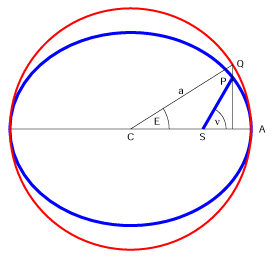
\includegraphics[width=0.5\hsize]{ellips2.png}
  \caption{Geometric interpretation of the eccentric anomaly (E)}
\end{figure}

\noindent
The relationship between orbit radius r and eccentric anomaly E is given by
\[ r = a(1-e \cos E) \]

\noindent
The relationship between true anomaly $\nu$ and E is given by
\[ \tan \frac{\nu}{2} = \sqrt{ \frac{1+e}{1-e}} \tan \frac{E}{2} \]

\noindent
With these equations, position P can be calculated when eccentric anomaly E is known. E is calculated for a given time t by solving \textit{Kepler's equation}.


\subsubsection{Kepler's equation}
Consider a vector rotating around C at constant angular velocity n, given by the orbiter's mean motion. If the vector passes A at time $t_{0}$, then its angle with A at time t is given by
\[ M(t) = n(t-t_0) \]

\noindent
M is called the \textit{mean anomaly}. Kepler's equation defines a relation between mean anomaly M and eccentric anomaly E:
\[ E(t) - e \sin E(t) = M(t) = n(t-t_0) \]

\noindent
It cannot be solved for E in closed form, and must generally be solved iteratively.

\end{document}
